% This file was created with tikzplotlib v0.10.1.post13.
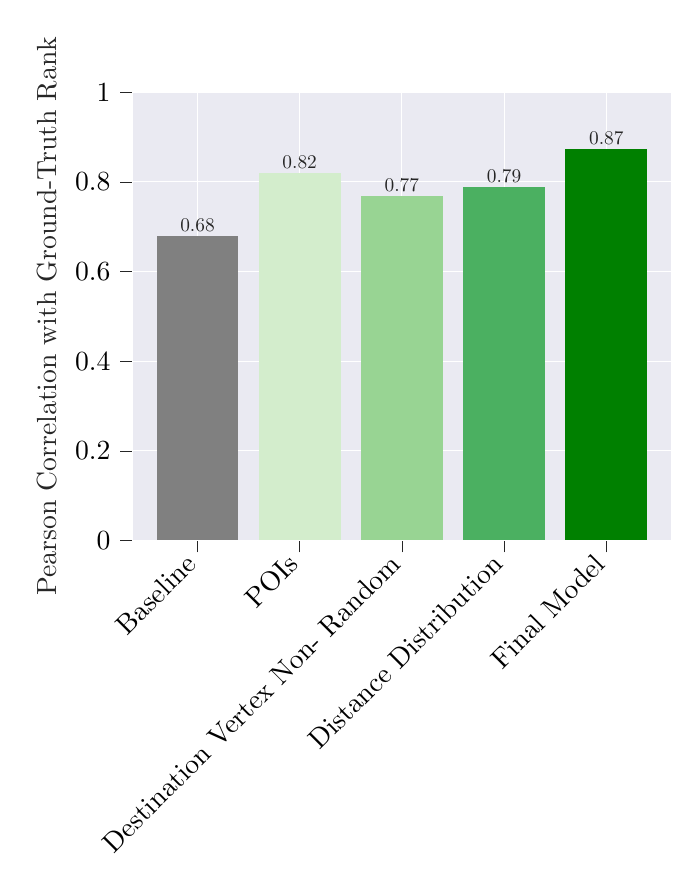
\begin{tikzpicture}

\definecolor{darkseagreen152212147}{RGB}{152,212,147}
\definecolor{darkslategrey38}{RGB}{38,38,38}
\definecolor{gainsboro211237204}{RGB}{211,237,204}
\definecolor{green}{RGB}{0,128,0}
\definecolor{grey}{RGB}{128,128,128}
\definecolor{lavender234234242}{RGB}{234,234,242}
\definecolor{mediumseagreen7517697}{RGB}{75,176,97}

\begin{axis}[
axis background/.style={fill=lavender234234242},
axis line style={white},
tick align=outside,
tick pos=left,
x grid style={white},
xmajorgrids,
xmin=-0.64, xmax=4.64,
xtick style={color=darkslategrey38},
xtick={0,1,2,3,4},
xticklabel style={rotate=45.0,anchor=east},
xticklabels={Baseline,POIs,Destination
Vertex Non-
Random,Distance
Distribution,Final Model},
y grid style={white},
ylabel=\textcolor{darkslategrey38}{Pearson Correlation with Ground-Truth Rank},
ymajorgrids,
ymin=0, ymax=1,
ytick style={color=darkslategrey38}
]
\draw[draw=none,fill=grey,line width=0.12pt] (axis cs:-0.4,0) rectangle (axis cs:0.4,0.678676181882812);
\draw[draw=none,fill=gainsboro211237204,line width=0.12pt] (axis cs:0.6,0) rectangle (axis cs:1.4,0.820551712217371);
\draw[draw=none,fill=darkseagreen152212147,line width=0.12pt] (axis cs:1.6,0) rectangle (axis cs:2.4,0.768360496661662);
\draw[draw=none,fill=mediumseagreen7517697,line width=0.12pt] (axis cs:2.6,0) rectangle (axis cs:3.4,0.789175316652419);
\draw[draw=none,fill=green,line width=0.12pt] (axis cs:3.6,0) rectangle (axis cs:4.4,0.872738754474632);
\draw (axis cs:0,0.688676181882812) node[
  scale=0.7,
  anchor=base,
  text=darkslategrey38,
  rotate=0.0
]{0.68};
\draw (axis cs:1,0.830551712217371) node[
  scale=0.7,
  anchor=base,
  text=darkslategrey38,
  rotate=0.0
]{0.82};
\draw (axis cs:2,0.778360496661662) node[
  scale=0.7,
  anchor=base,
  text=darkslategrey38,
  rotate=0.0
]{0.77};
\draw (axis cs:3,0.799175316652419) node[
  scale=0.7,
  anchor=base,
  text=darkslategrey38,
  rotate=0.0
]{0.79};
\draw (axis cs:4,0.882738754474632) node[
  scale=0.7,
  anchor=base,
  text=darkslategrey38,
  rotate=0.0
]{0.87};
\end{axis}

\end{tikzpicture}
